\chapter{Knihovna pro práci s regulárními výrazy}\label{sec:Implementation1}

Jako prvotní myšlenka před tvorbou samotné vizualizace, jsem měl úvahu o použití knihovny, 
která by mi umožňovala zpracovávat regulární výrazy.
Sice implementace regulárních výrazů se nachází v samotné specifikaci JavaScriptu,
ale ta mi neumožňuje získat informaci o samotném vyhledávání.
Po prozkoumání, zda-li existují řešení, která by vyhovovala této práci, 
jsem uznal za vhodné, vytvořit vlastní implementaci v podobě této knihovny.
Nenaleznul jsem totiž řešení, které by bylo dostatečně flexibilní a 
zároveň lehce integrovatelné do programovacího jazyku TypeScript.
Sice vlastní implementace je pracná, ale jelikož chci mít co nejvyšší kontrolu nad výslednou strukturou, 
tak je toto řešení pro tuto aplikaci asi nejvhodnější. 

V této části práce se pokusím vysvětlit, jak je naimplementována tato knihovna \ref{sec:Imp1LayoutReal}, 
jaké problémy se ukázali při vývoji a její výhody a nevýhody. % TODO: references

\section{Rozvržení a realizace}\label{sec:Imp1LayoutReal}

Vstupní třídou, pro tuto knihovnu je \textbf{Regexer}. 
Slouží jako spojující a zároveň obsluhující třída. 
Zároveň poskytuje rozhraní této knihovny.
Dále si drží důležité informace, které souvisí s aktuálním regulárním výrazem.
\textbf{RegexMatch} je třída, jejíž instance je výsledkem vyhledávání zadaným výrazem.
Její data jsou soukromá, ale umožňuje je procházet pomocí svých metod.
Jedna instance teto třídy, je ekvivalentní jednomu vyhledání v textu.
Data této třídy jsou generována třídou \textbf{MatchBuilder}.
Instance této třídy existuje jen ve chvíli, kdy probíhá vyhledávání v zadaném řetězci.
Poskytuje rozhraní, které umožňuje přidávat stavy, s tím že může s těmito daty manipulovat.
Tento objekt je pak držený v tříde \textbf{MatcherInternal}, 
která má za ůkol, průchod zadaným řetězcem, pro konkrétní výraz.
Tato třída, je izolována a není dostupná z vnější, jak její jméno (internal) napovídá.
Obsahuje hlavní logickou část průchodu nedeterministickým automatem.
Naopak třídou, která poskytuje vyditelné rozhraní a volá metody třídy MatcherInternal je \textbf{Matcher}.
Její rozhraní je poskytováno třídě Regexer.
Jako poslední struktura, která stojí za zmínku, je \textbf{Stack}.
Stack nebo-li zásobník, je velmi důležitou součástí vyhledávání.
Zásobník je totiž struktura, která mi dovoluje se zbavit rekurzivního volání funkce.
Rekurze obecně vede k pomalejšímu chodu programu a nelze ji jednoduše pozastavit v jakémkoliv čase.
Sice rozhraní pole v JS je připraveno na funkcionalitu zásobníku, 
ale nezaručuje programátorovi daná pravidla pro zásobník. 
Z tohoto důvodu jsem zvolil jednoduchou implementaci zásobníku, 
která omezuje manipulaci s základním polem, na operace určené pro zásobník.

% TODO: add RegexParser

Vztahy mezi jednotlivými třídami, lze vidět na obrázku \ref{fig:ARCH_RGXR}. 
Myslím si že je vhodné poukázat na obalující blok \textbf{MatchingWorker}.
Jedná se o vstupní soubor vedlejšího vlákna, který slouží pro asynchroní komunikaci s hlavním vláknem.


% Je-li vytvořena instance této třídy, je potřeba parsnout zadaný regulární výraz, pomocí metody \textbf{parse}.
% Regexer, jako řídící třída zavolá RegexParser, který dokáže zpracovat textovou podobu regulárního výrazu na strukturu AST a NKA.
% TODO ^ update, change location probbably

\begin{figure}[!h]
	\centering
	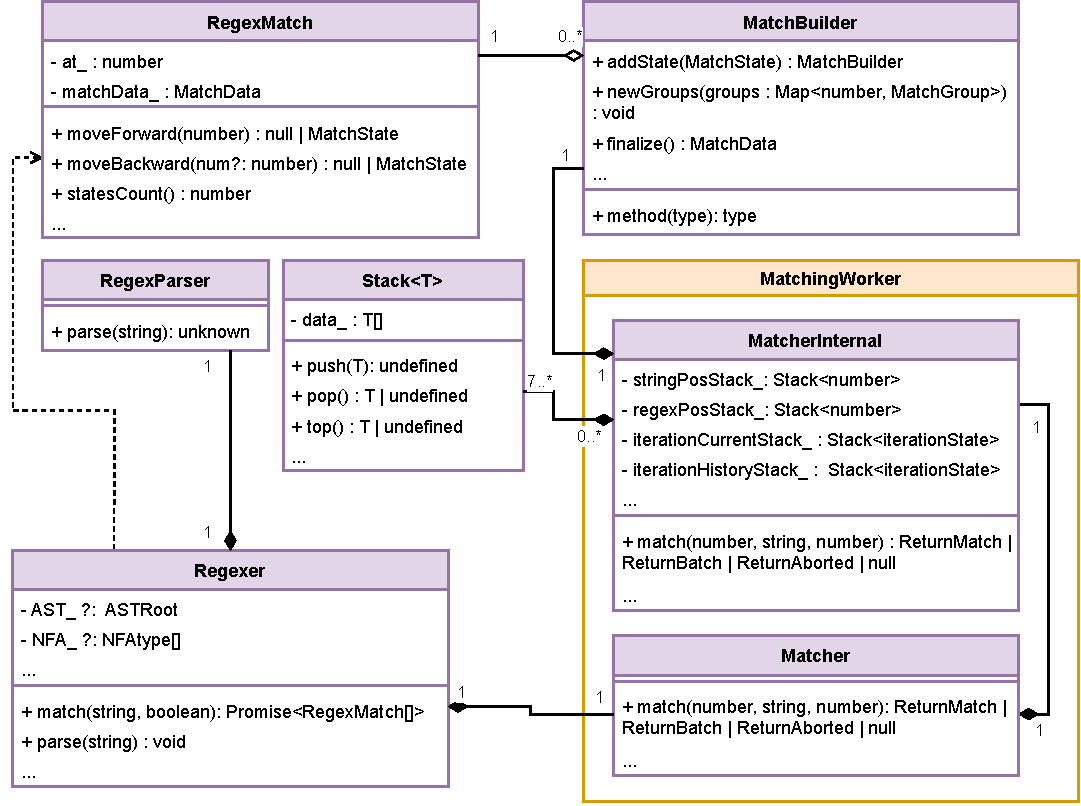
\includegraphics[width=0.9\textwidth]{Figures/UML_RGXR.pdf}
	\caption{Třídní diagram části knihovny pro práci s regulárními výrazy}
	\label{fig:ARCH_RGXR}
\end{figure}


\subsection*{Parser regulárních výrazů}

Jak již bylo zmíněno, pro parsování regulárních výrazu jsem použil bezkontextovou gramatiku Peggy.
Jedná se o pokračování projektu pegjs, ale ten se již dlouho nevyvíjí. 
Jelikož tato knihovna je stále aktualizována a má velkou podporu vývojářů, tak jsem zvolil její využití pro tuto práci.

\subsection*{Využití vlákna pro vyhledávání}
Nedílnou součástí této knihovny je \textbf{paralelní zpracování} v podobě balíčku threads.js.
Balíček byl již zmíněn v kapitole \ref{sec:USEDtech}.
Toto využití nám dovoluje složité operace přesunout tak, aby hlavní vlákno nebylo zatíženo.
Vlákna nám sice umožňují efektivnější rozložení náročných programů, ale také mají svá ůskalí.

JavaScript je standartně vykonáván na jediném vlákně a tak neexistuje stejné více vláknové programování, jako v jiných jazycích.
Jelikož chci docílit podobného výsledku, musím spustit paralelní program, 
který komunikuje s hlavním vláknem, pomocí zpráv.

S volbou vývojového prostředí vscode, byla nutnost splnit podmínky stanovené pro práci s web workery, v souladu s jejich API. 
Podmínkou totiž je, nutnost mít zdrojový kód workeru přímo vložený ve zdrojovém kódu hlavního vlákna.
To znamená, že worker nesmí být přímo načítaný, z adresáře rozšíření.
Avšak tato nutnost, je komplikovaná a proto následovně vysvětlím, jak jsem tento problém řešil.
Všechny závislosti, které worker má musí být součástí jednoho výsledného souboru.
To je docíleno tím, že přeložím soubor pomocí webpacku, který vytvoří jeden výsledný soubor.
Pokud by chtěl někdo využít této knihovny, v rámci prostředí NodeJS nebo Prohlížeče, 
tak tento překlad probíhá dvakrát pro obě prostředí.
Tento soubor může následně být vložen přímo do zdrojového kódu.
Pokud prostředí, které využívá tuto knihovnu má webpack, 
může využít loaderu, který jsem pro tuto knihovnu napsal. 
Ten dokáže v místě kde je worker volaný, vložit jeho zdrojový kód, v rámci textového řetězce.
Výsledkem je worker, který je vložený ve zdrojovém kódě hlavního vlákna.

%TODO: přidat odkaz na vscode api jako citaci

\endinput